% Vector redraw of SystemDesign.png (Appendix figure fig:system-design).
% Same three panels, boxes and arrows as the original raster; fixes its baked-in
% typos ("Singie LLM", "Eamings Call"). Build: pdflatex system_design.tex -> system_design.pdf
\documentclass[tikz,border=4pt]{standalone}
\usepackage[T1]{fontenc}
\usepackage[scaled]{helvet}
\renewcommand{\familydefault}{\sfdefault}
\usetikzlibrary{positioning,arrows.meta,shapes.symbols,fit,calc}

\definecolor{dblue}{HTML}{2F5597}
\definecolor{navy}{HTML}{1F3864}
\definecolor{teal}{HTML}{1B8A94}
\definecolor{tealsoft}{HTML}{B9DCDD}
\definecolor{grp}{HTML}{D6DCEB}
\definecolor{cmacro}{HTML}{6A9A3A}
\definecolor{cvalue}{HTML}{D4A017}
\definecolor{crisk}{HTML}{2F5597}
\definecolor{ctech}{HTML}{E07B39}
\definecolor{ttl}{HTML}{1F3864}

\begin{document}
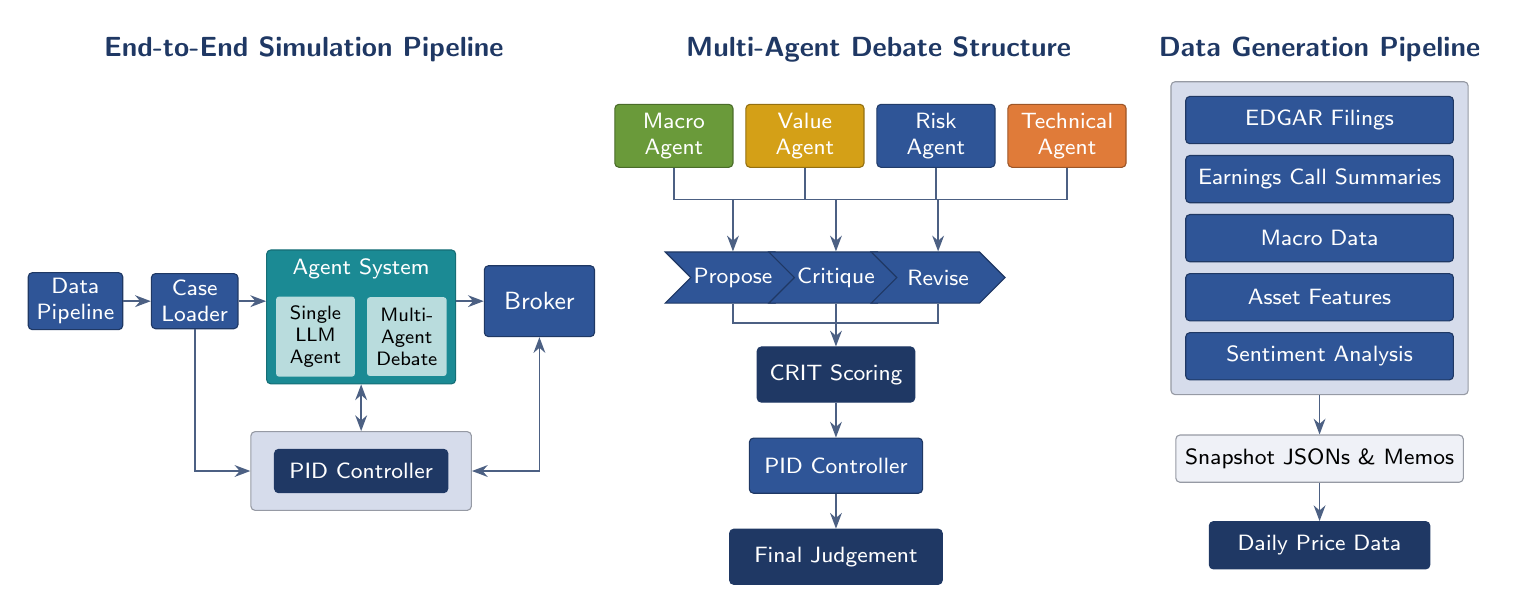
\begin{tikzpicture}[
    font=\footnotesize,
    b/.style={draw=navy, fill=dblue, text=white, rounded corners=1.5pt, align=center,
      minimum height=7mm, inner sep=2pt, line width=0.4pt},
    ag/.style={b, fill=#1, draw=#1!70!black, minimum width=15mm, minimum height=8mm},
    ch/.style={signal, signal to=east, signal from=west, fill=dblue, draw=navy, text=white,
      minimum height=6.5mm, minimum width=17mm, inner sep=1pt},
    a/.style={-{Stealth[length=2mm]}, draw=navy!80, line width=0.6pt},
    t/.style={font=\normalsize\bfseries, text=ttl},
  ]
  %% ---------------- panel 1: end-to-end simulation pipeline
  \node[t] at (2.9, 3.2) {End-to-End Simulation Pipeline};
  \node[b, minimum width=12mm] (dp) at (0,0) {Data\\Pipeline};
  \node[b, minimum width=11mm, right=3.5mm of dp] (cl) {Case\\Loader};
  \node[draw=teal!80!black, fill=teal, rounded corners=1.5pt, minimum width=24mm, minimum height=17mm,
        right=3.5mm of cl, yshift=-2mm] (as) {};
  \node[text=white, anchor=north] at (as.north) {Agent System};
  \node[fill=tealsoft, rounded corners=1pt, align=center, font=\scriptsize, minimum width=10mm,
        minimum height=10mm] at ($(as.center)+(-5.8mm,-2.5mm)$) {Single\\LLM\\Agent};
  \node[fill=tealsoft, rounded corners=1pt, align=center, font=\scriptsize, minimum width=10mm,
        minimum height=10mm] at ($(as.center)+(5.8mm,-2.5mm)$) {Multi-\\Agent\\Debate};
  \node[b, minimum width=14mm, minimum height=9mm, font=\small, right=3.5mm of as, yshift=2mm] (br) {Broker};
  \node[draw=grp!70!black, fill=grp, rounded corners=1.5pt, minimum width=28mm, minimum height=10mm]
        (pidg) at ($(as.south)+(0,-11mm)$) {};
  \node[b, fill=navy, minimum width=22mm, minimum height=5.5mm] (pid) at (pidg.center) {PID Controller};
  \draw[a] (dp) -- (cl);
  \draw[a] (cl.east) -- (cl.east -| as.west);
  \draw[a] (as.east |- br.west) -- (br.west);
  \draw[{Stealth[length=2mm]}-{Stealth[length=2mm]}, draw=navy!80, line width=0.6pt] (as.south) -- (pidg.north);
  \draw[a] (cl.south) |- (pidg.west);
  \draw[{Stealth[length=2mm]}-{Stealth[length=2mm]}, draw=navy!80, line width=0.6pt]
        (pidg.east) -| (br.south);

  %% ---------------- panel 2: multi-agent debate structure
  \begin{scope}[xshift=7.6cm]
  \node[t] at (2.6, 3.2) {Multi-Agent Debate Structure};
  \node[ag=cmacro] (m) at (0,2.1) {Macro\\Agent};
  \node[ag=cvalue, right=1.5mm of m] (v) {Value\\Agent};
  \node[ag=crisk,  right=1.5mm of v] (r) {Risk\\Agent};
  \node[ag=ctech,  right=1.5mm of r] (tq) {Technical\\Agent};
  \node[ch] (pr) at (0.75,0.3) {Propose};
  \node[ch, right=-1mm of pr] (cr) {Critique};
  \node[ch, right=-1mm of cr] (rv) {Revise};
  \draw[draw=navy!80, line width=0.6pt] (m.south) |- ($(tq.south)+(0,-4mm)$) -- (tq.south);
  \draw[draw=navy!80, line width=0.6pt] (v.south) -- ++(0,-4mm);
  \draw[draw=navy!80, line width=0.6pt] (r.south) -- ++(0,-4mm);
  \foreach \n in {pr,cr,rv} \draw[a] (\n.north |- {$(m.south)+(0,-4mm)$}) -- (\n.north);
  \node[b, fill=navy, minimum width=20mm] (crit) at ($(cr.south)+(0,-9mm)$) {CRIT Scoring};
  \node[b, minimum width=22mm] (pid2) at ($(crit.south)+(0,-8mm)$) {PID Controller};
  \node[b, fill=navy, minimum width=27mm] (fj) at ($(pid2.south)+(0,-8mm)$) {Final Judgement};
  \draw[draw=navy!80, line width=0.6pt] (pr.south) |- ($(crit.north)+(0,3mm)$) -| (rv.south);
  \draw[a] (cr.south) -- (crit.north);
  \draw[a] (crit) -- (pid2);
  \draw[a] (pid2) -- (fj);
  \end{scope}

  %% ---------------- panel 3: data generation pipeline
  \begin{scope}[xshift=14.3cm]
  \node[t] at (1.5, 3.2) {Data Generation Pipeline};
  \foreach \lab/\y [count=\i] in {EDGAR Filings/2.3, Earnings Call Summaries/1.55, Macro Data/0.8,
                                  Asset Features/0.05, Sentiment Analysis/-0.7}
    \node[b, minimum width=34mm, minimum height=6mm] (d\i) at (1.5,\y) {\lab};
  \node[draw=grp!70!black, fill=grp, rounded corners=1.5pt, inner sep=1.8mm, fit=(d1)(d5)] (grpbox) {};
  \foreach \lab/\y [count=\i] in {EDGAR Filings/2.3, Earnings Call Summaries/1.55, Macro Data/0.8,
                                  Asset Features/0.05, Sentiment Analysis/-0.7}
    \node[b, minimum width=34mm, minimum height=6mm] at (1.5,\y) {\lab};
  \node[draw=grp!70!black, fill=grp!40, text=black, rounded corners=1.5pt, minimum width=34mm,
        minimum height=6mm] (snap) at (1.5,-2.0) {Snapshot JSONs \& Memos};
  \node[b, fill=navy, minimum width=28mm, minimum height=6mm] (px) at (1.5,-3.1) {Daily Price Data};
  \draw[a] (grpbox.south) -- (snap.north);
  \draw[a] (snap) -- (px);
  \end{scope}
\end{tikzpicture}
\end{document}
